\documentclass[11pt,varwidth=\maxdimen]{standalone}
%\documentclass{article}
\usepackage[english]{babel}	
\usepackage[utf8]{inputenc}	% Allows for writing special charachters in the tex-file 

\usepackage{amsfonts,amsmath,amssymb,bm,mathrsfs,mathtools,dsfont} 	% Standard mathematics 

\newcommand{\braces}[1]{\left\lbrace #1 \right\rbrace}
\newcommand{\brackets}[1]{\left( #1 \right)}
\newcommand{\squarebrackets}[1]{\left[ #1 \right]} 
\newcommand{\angles}[1]{\left\langle #1\right\rangle}
\newcommand{\abs}[1]{\left\lvert #1 \right\rvert}
\newcommand{\norm}[1]{\left\Vert #1 \right\Vert}

\usepackage[dvipsnames,table]{xcolor}
\definecolor{rmp}{RGB}{41, 43, 133}
\definecolor{myblue}{rgb}{0.24, 0.36, 0.44}
\definecolor{mygreen}{rgb}{0.367, 0.473, 0.0}
\newcommand{\myBlue}[0]{RoyalBlue}
\newcommand{\myGreen}[0]{OliveGreen}
\newcommand{\myRed}[0]{OrangeRed}
\newcommand{\myYellow}[0]{Goldenrod}


\usepackage{tikz}
\usetikzlibrary{positioning,shapes,calc,arrows.meta}
\newcommand{\coord}[4]{({(#1)+(#3)*cos(#4)},{(#2)+(#3)*sin(#4)})}


\newcommand{\sscript}[1]{{\scriptscriptstyle \mathrm{#1}}}
\newcommand{\EFT}{\sscript{EFT}}


% % % % % % Commands % % % % % % %

\begin{document}

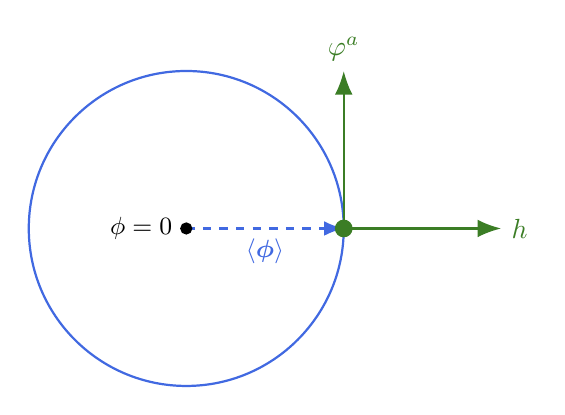
\begin{tikzpicture}
	\tikzset{baseline=(c.base)}
	\node (0,0) (c) {};
	\draw[\myBlue, thick] (0,0) circle (2);
	\draw[\myBlue, thick, dashed, -{Latex[length=2.5mm]}] (0,0) -- node[anchor=north] {\small $\langle\boldsymbol{\phi}\rangle$} (2,0);
	\filldraw[\myGreen] (2,0) circle (3pt);
	\draw[\myGreen, thick, -{Latex[length=3mm]}] (2,0) -- (4,0) node[right] {$h$};
	\draw[\myGreen, thick, -{Latex[length=3mm]}] (2,0) -- (2,2) node[above] {$\varphi^a$};
	\filldraw[black] (0,0) circle (2pt) node[anchor=east] {\small $\phi=0$\,};
\end{tikzpicture}
\\[0.2cm]
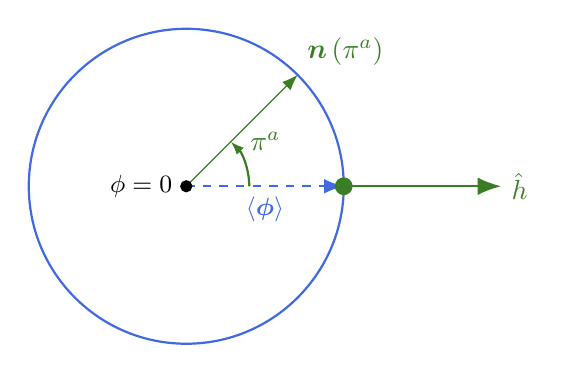
\begin{tikzpicture}
	\tikzset{baseline=(c.base)}
	\node (0,0) (c) {};
	\draw[\myBlue, thick] (0,0) circle (2);
	\draw[\myBlue, thick, dashed, -{Latex[length=2.5mm]}] (0,0) -- node[anchor=north] {\small $\langle\boldsymbol{\phi}\rangle$} (2,0);
	\filldraw[\myGreen] (2,0) circle (3pt);
	\draw[\myGreen, thick, -{Latex[length=3mm]}] (2,0) -- (4,0) node[right] {$\hat{h}$};
	\draw[\myGreen, -{Latex[length=2mm]}] (0,0) -- (1.41421,1.41421) node[above right] {$\boldsymbol{n}\brackets{\pi^a}$};
	\draw[\myGreen, thick, -{Latex[length=1.7mm]}] (0.8,0) arc (0:45:8mm) node[right] {$~\pi^a$};
	\filldraw[black] (0,0) circle (2pt) node[anchor=east] {\small $\phi=0$\,};
\end{tikzpicture}

\end{document}